\documentclass[uplatex]{jsarticle}
\usepackage{resume}
\usepackage{udline}
\usepackage{comment}

\pagestyle{plain}

\begin{document}
\twocolumn[
    \beginheader{コンピュータサイエンス学部 中中間発表}{2026}{6}{19}{井上 研究室}
    \title{VR上での近距離のヒットストップへの違和感低減手法}
    \author{C0B23094 武田 明良 (Akira Takeda)}
    \endheader
]

\vspace{3mm}
\setcounter{page}{1}  % このページ数は自分の順番が決まった時に変える

\section{はじめに}
ゲームという娯楽コンテンツは,駒やカードを用いる卓上のアナログなものから始まり,コンピュータを用いたビデオゲームへと進化した.現代ではビデオゲームの進化系としてゴーグル型のディスプレイで仮想空間を投影して楽しむVRゲームが誕生した.このVRゲームにはこれまでのゲーム制作で培われてきた技術が多く使われている.

これまでビデオゲームは没入感を高める技術を様々生み出し,多くのゲームに活用してきた.その中の一つに「ヒットストップ」という技術が存在する.「ヒットストップ」とは,パンチや爆発など,衝撃が発生したタイミングで映像を一瞬停止させて,プレイヤーにその衝撃力を感じさせる映像技術であり,大乱闘スマッシュブラザーズやストリートファイターなど,大きなアクションや攻撃を用いるゲームで頻繁に使用されている.

このヒットストップという技術はVR上でも従来のビデオゲームと同様の効果を発揮することが明らかになっている.\cite{HitStop}しかし,VRゲームでは従来のビデオゲームのようなヒットストップは見られない.

VR上では,映像の急激な変化が違和感をもたらすことが原因として挙げられる.\cite{InstantChange}ヒットストップは急激な映像の変化を起こしてしまい,衝撃提示などの正の要素より,不自然さなどの負の要素が強くなってしまう.

また,VRゲームでの操作は従来のビデオゲームと比べて,より直感的である.この状況下でヒットストップを発生させると,VR上の手や首の動きが,実際の身体の動きとずれてしまい,これが違和感をもたらす要因である可能性が高い.実際,WiiSportsResortというビデオゲームでは,コントローラーを振って剣を操作するゲームがあるが,このゲームにおいてはヒットストップは発生しないようになっている.

しかし,ヒットストップは特別な機材を必要とせずに衝撃力を提示できる技術であり,完全な代替技術が存在しない.没入感を高めることを目的とした場合,最も簡単に実装でき,既存の全ての機材で使用できる技術だ.

そこで本研究では,ヒットストップがもたらす違和感だけを低減させ,衝撃力を提示させられる手法として,非連動部位停止手法を提案する。(\figref{fig:unlinkHitstop})非連動部位停止手法とは,現実の動作と連動していない,VR上にのみ存在する部位だけヒットストップを発生させる手法だ,ヒットストップは発生させたのが自身か他ユーザかで感じる違和感に差があることが分かっている.\cite{MultiPlayerHitStop}

\begin{figure}
    \centering
    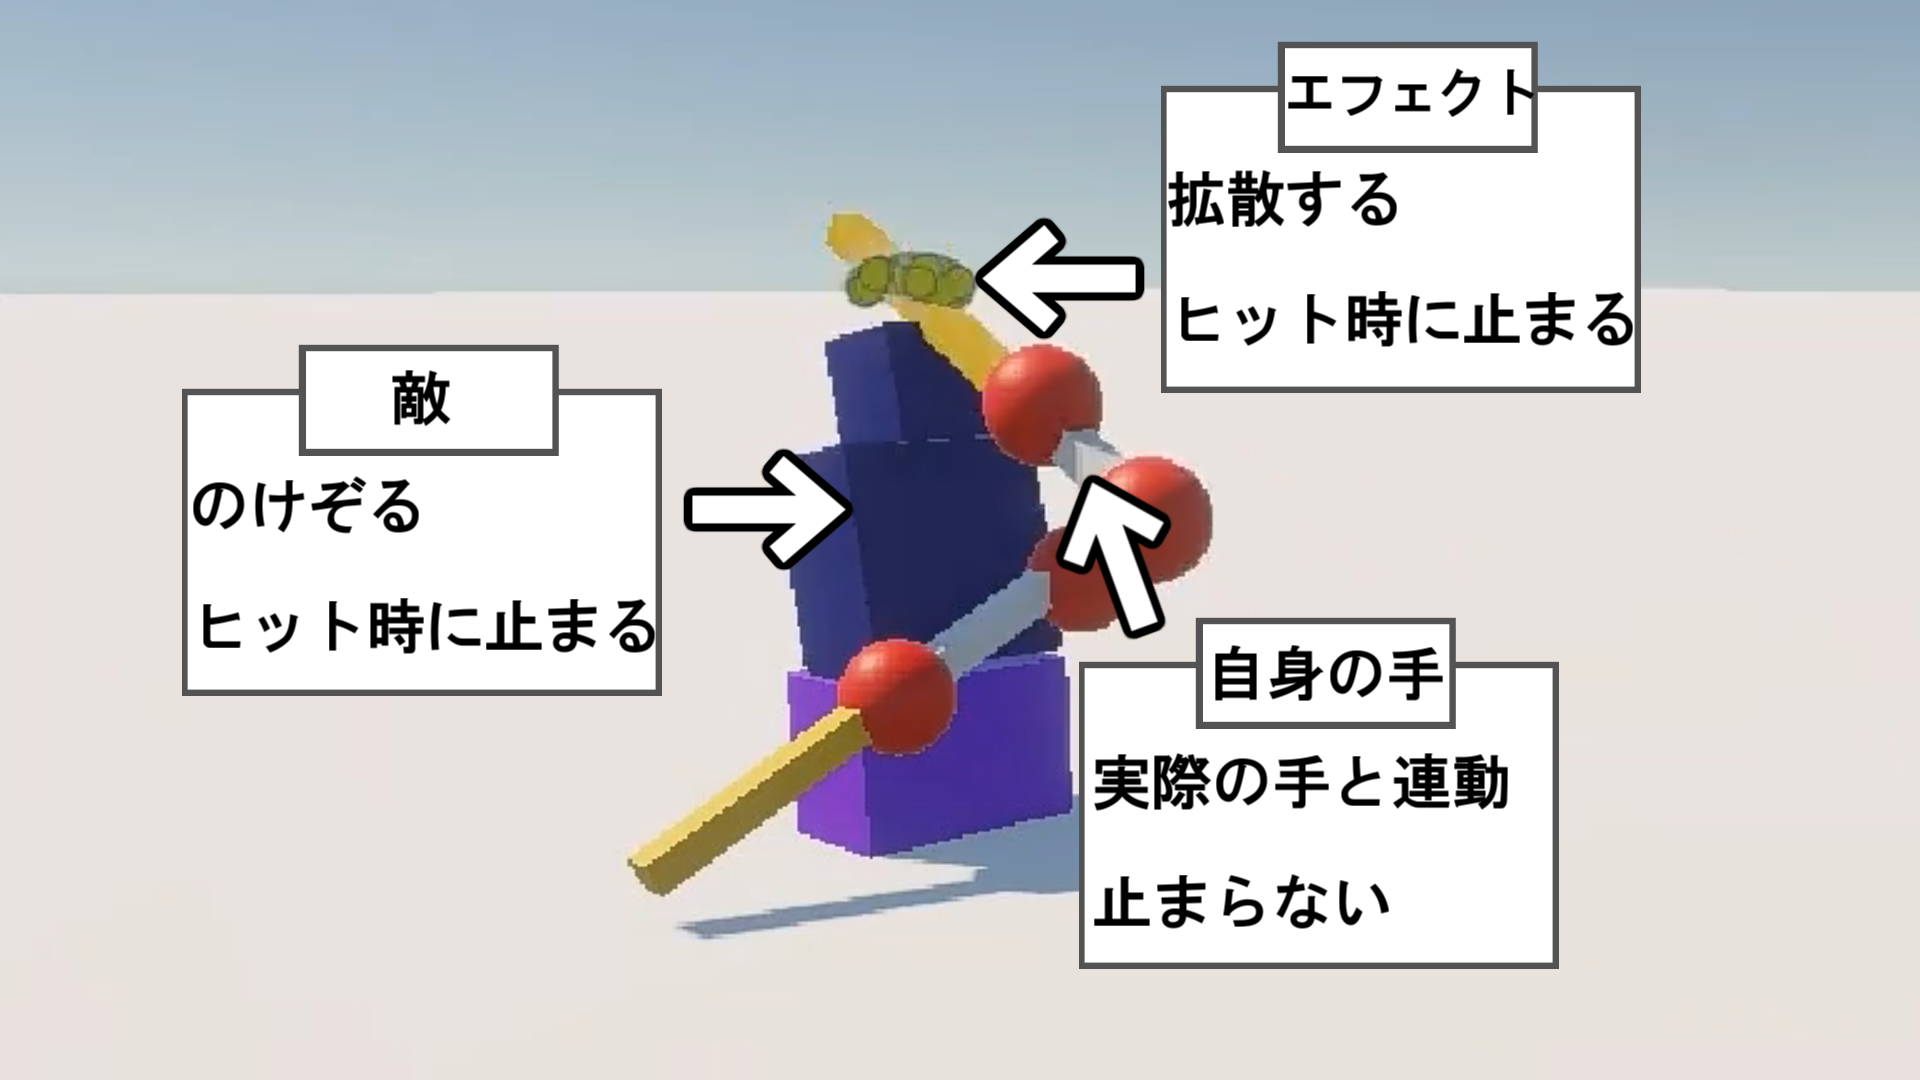
\includegraphics[width=1.0\linewidth]{NewMethodHitStop.png}
    \caption{非連動部位停止手法}
    \label{fig:unlinkHitstop}
\end{figure}

\begin{figure}[h]
    \centering
    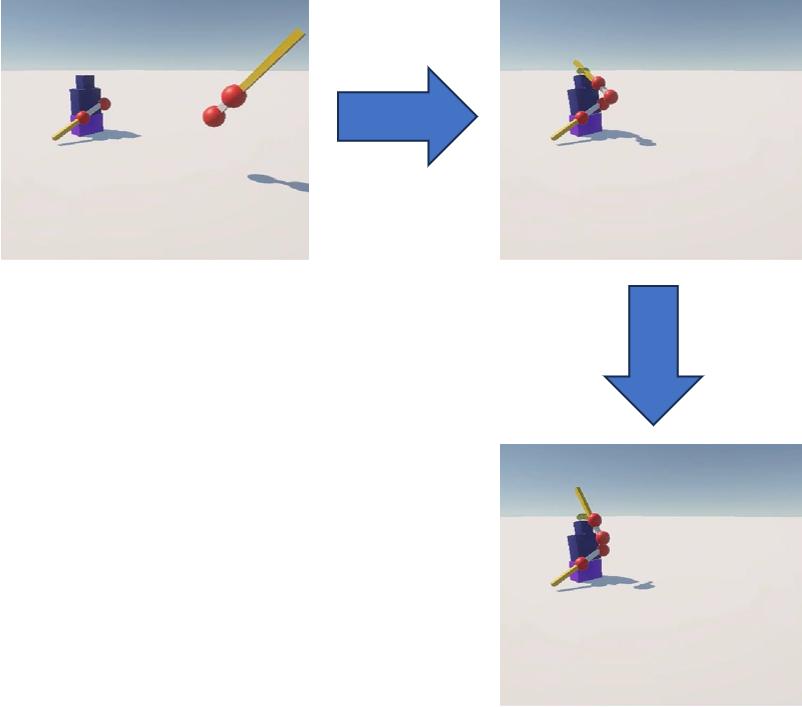
\includegraphics[width=0.7\linewidth]{UnlinkHitstop.png}
    \caption{局所発生の例}
    \label{fig:unlink}
\end{figure}

\section{ヒットストップ局所発生システム}
\subsection{システム概要}
本研究は剣道の面打ちを実験タスクとして設定しているため,今後の説明は剣道の面打ちを前提としている.システムは,相手に面がヒットした時にエフェクトが出現すると同時に,ヒットストップが発生するシステムだ.


\subsection{局所発生}
本システムの特徴として,ヒットストップが発生する際に停止する部位を事前に選択することができる.\figref{fig:unlink}はエフェクトと敵をヒットストップ発生部位として選択した時のフローだ.
\subsection{振動}
先行研究より,VR上でのヒットストップはコントローラーの振動が無いとむしろ違和感を助長する要素になる.\cite{HitStop}そのため,本システムでは先行研究と同様にヒットストップの発生時に,発生部位に関わらず200msコントローラーを振動させる.

\section{実装}
現時点ではヒットストップ局所発生システムの動きをデモンストレーションするアニメーションのみ作成している.

\begin{figure}[h]
    \centering
    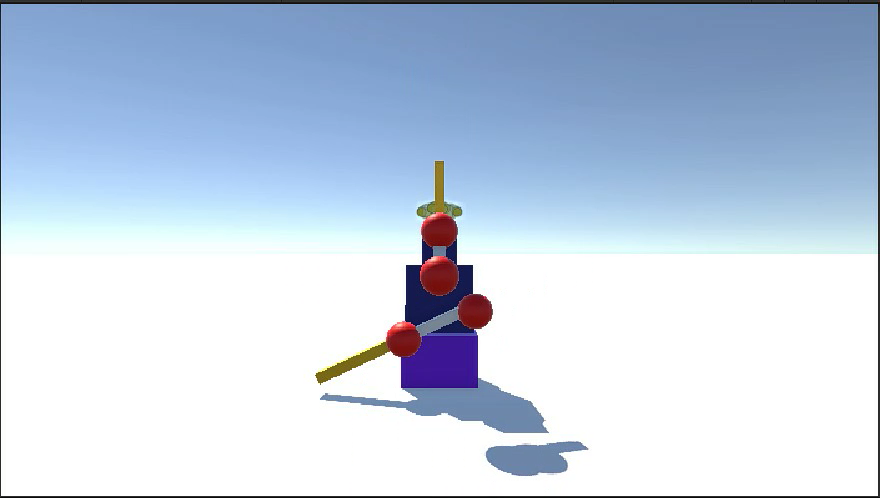
\includegraphics[width=0.5\linewidth]{一人称デモ.png}
    \caption{一人称視点のデモアニメーション}
    \label{fig:fp}
\end{figure}

\begin{figure}[h]
    \centering
    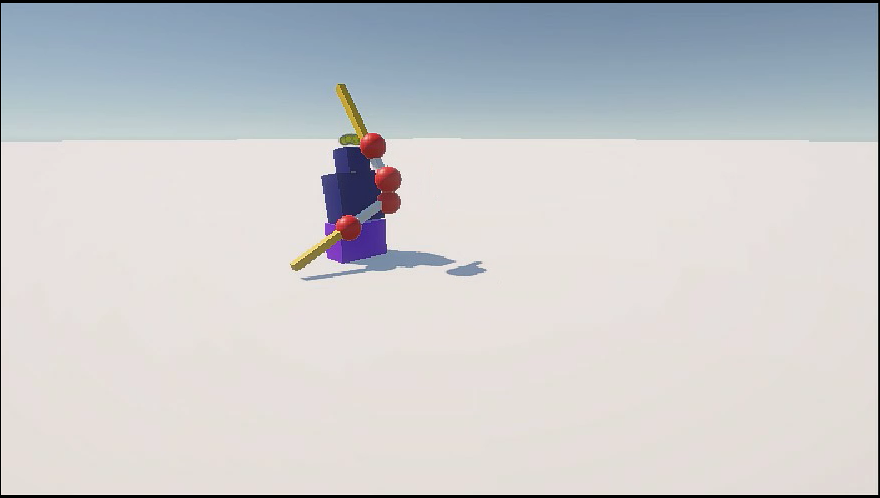
\includegraphics[width=0.5\linewidth]{三人称デモ.png}
    \caption{三人称視点のデモアニメーション}
    \label{fig:tp}
\end{figure}

\section{評価}
本実験はアンケートによる主観的情報を評価データとして扱う.停止させる部位を変えて面を打つ度に違和感と体験の質に関するアンケートを行い,その結果から違和感の低下と体験の質の向上を最も両立できたパターンから考察する.

先行研究ではVRでの体験の質を心拍数や血圧などのバイタルサインから読み取ることは難しいと述べられている.\cite{TimeflowAndQoE}

\section{おわりに}
\subsection{まとめ}
本研究では,ヒットストップによって生じる違和感を減少させつつ,衝撃力を提示させる手法として,ヒットストップが発生する部位を絞り,現実の身体と連動しない部位でだけヒットストップを発生させる手法を提案した.

\subsection{課題}
現在想定している実験タスクは,剣道の面打ちのみであり,道具を用いない場合や,遠距離で衝撃が発生した場合など,そのまま今回の結果を流用してはいけない可能性のあるケースが多い.

現時点で考えている評価方法では,主観的な数値しか集められないため,結果が個人差程度の誤差しかない危険性がある.

\subsection{今後について}
中間発表までに実験を行い,実際にデータを集めた結果から,データの追加収集や,タスクの種類を変えての実験を行いたい.

\bibliographystyle{junsrt}
\bibliography{ref}
\end{document}
